% This is a Basic Assignment Paper but with like Code and stuff allowed in it. 

\documentclass[11pt]{article}

% Preamble

\usepackage[margin=1in]{geometry}
\usepackage{amsfonts, amsmath, amssymb}
\usepackage{fancyhdr, float, graphicx}
\usepackage[utf8]{inputenc} % Required for inputting international characters
\usepackage[T1]{fontenc} % Output font encoding for international characters
\usepackage{fouriernc} % Use the New Century Schoolbook font
\usepackage[nottoc, notlot, notlof]{tocbibind}
\usepackage{listings}
\usepackage{xcolor}
\usepackage{karnaugh-map}
\usepackage{pdfpages}

\definecolor{codegreen}{rgb}{0,0.6,0}
\definecolor{codegray}{rgb}{0.5,0.5,0.5}
\definecolor{codepurple}{rgb}{0.58,0,0.82}
\definecolor{backcolour}{rgb}{0.95,0.95,0.92}

\lstdefinestyle{mystyle}{
    backgroundcolor=\color{backcolour},   
    commentstyle=\color{codegreen},
    keywordstyle=\color{magenta},
    numberstyle=\tiny\color{codegray},
    stringstyle=\color{codepurple},
    basicstyle=\ttfamily\footnotesize,
    breakatwhitespace=false,         
    breaklines=true,                 
    captionpos=b,                    
    keepspaces=true,                 
    numbers=left,                    
    numbersep=5pt,                  
    showspaces=false,                
    showstringspaces=false,
    showtabs=false,                  
    tabsize=2
}

\lstset{style=mystyle}

% Header and Footer
\pagestyle{fancy}
\fancyhead{}
\fancyfoot{}
\fancyhead[L]{\textit{\Large{DECA Active Learning}}}
%\fancyhead[R]{\textit{something}}
\fancyfoot[C]{\thepage}
\renewcommand{\footrulewidth}{1pt}



% Other Doc Editing
% \parindent 0ex
%\renewcommand{\baselinestretch}{1.5}

\begin{document}

\begin{titlepage}
	\centering

	%---------------------------NAMES-------------------------------

	\huge\textsc{
		MIT World Peace University
	}\\

	\vspace{0.75\baselineskip} % space after Uni Name

	\LARGE{
		Digital Electronics and Computer Architecture\\
		Second Year B. Tech, Semester 1
	}

	\vfill % space after Sub Name

	%--------------------------TITLE-------------------------------

	\rule{\textwidth}{1.6pt}\vspace*{-\baselineskip}\vspace*{2pt}
	\rule{\textwidth}{0.6pt}
	\vspace{0.75\baselineskip} % Whitespace above the title



	\huge{\textsc{
			4 Bit Adder and Subtracter using IC 7483
		}} \\



	\vspace{0.5\baselineskip} % Whitespace below the title
	\rule{\textwidth}{0.6pt}\vspace*{-\baselineskip}\vspace*{2.8pt}
	\rule{\textwidth}{1.6pt}

	\vspace{1\baselineskip} % Whitespace after the title block

	%--------------------------SUBTITLE --------------------------	

	\LARGE\textsc{
		Practical Report
	} % Subtitle or further description
	\vfill

	%--------------------------AUTHOR-------------------------------

	Prepared By
	\vspace{0.5\baselineskip} % Whitespace before the editors

	\Large{
		Krishnaraj Thadesar, PA20 \\
		Avipsa Ghorai, PA18\\
		Shivranjan Pathak, PA16\\
		Vaishnavi Powar, PA19\\
		Pratyush Choudhari, PA17\\
		Cyber Security and Forensics\\
		Batch A1
	}


	\vspace{0.5\baselineskip} % Whitespace below the editor list
	\today

\end{titlepage}


\tableofcontents
\thispagestyle{empty}
\clearpage


\setcounter{page}{1}
\section{Problem Statement}
\textit{To design and implement 4 bit Adder and Subtractor using IC 7483 parallel adder.}

\section{Components Used}
\begin{enumerate}
	\item 2 1.5 V AA Batteries or 3 Volt Power Source
	\item DIP Switch SPST x 4"
	\item DIP Switch DPST"
	\item Quad XOR gate"
	\item 4-Bit Adder"
	\item 5 Red LED"
	\item 220 Ω Resistor"
	\item 4 Blue LED"
	\item 4 Orange LED"
\end{enumerate}

\section{Truth Table of Involved Truth Tables}
\subsection{4 bit Full Adder}
\begin{figure}[H]
\centering
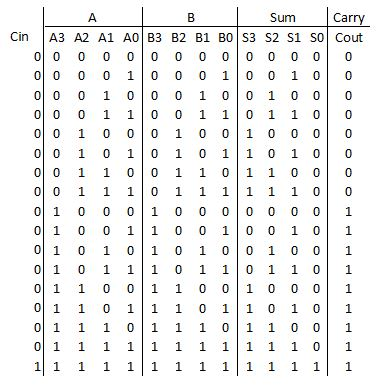
\includegraphics[scale=0.9]{4-bit-adder-Turth-Table.jpg}
\caption{}
\end{figure}
\subsection{Truth Table of 3 Bit Full Subtractor}
\begin{table}[H]
	\centering
	\begin{tabular}{|ccc|cc|}
		\hline
		\multicolumn{3}{|c|}{\textbf{Inputs}} & \multicolumn{2}{c|}{\textbf{Outputs}}                                                                             \\ \hline
		\multicolumn{1}{|c|}{\textbf{A}}      & \multicolumn{1}{c|}{\textbf{B}}       & \textbf{Borrow In} & \multicolumn{1}{c|}{\textbf{Diff}} & \textbf{Borrow} \\ \hline
		\multicolumn{1}{|c|}{0}               & \multicolumn{1}{c|}{0}                & 0                  & \multicolumn{1}{c|}{0}             & 0               \\ \hline
		\multicolumn{1}{|c|}{0}               & \multicolumn{1}{c|}{0}                & 1                  & \multicolumn{1}{c|}{1}             & 1               \\ \hline
		\multicolumn{1}{|c|}{0}               & \multicolumn{1}{c|}{1}                & 0                  & \multicolumn{1}{c|}{1}             & 1               \\ \hline
		\multicolumn{1}{|c|}{0}               & \multicolumn{1}{c|}{1}                & 1                  & \multicolumn{1}{c|}{0}             & 1               \\ \hline
		\multicolumn{1}{|c|}{1}               & \multicolumn{1}{c|}{0}                & 0                  & \multicolumn{1}{c|}{1}             & 0               \\ \hline
		\multicolumn{1}{|c|}{1}               & \multicolumn{1}{c|}{0}                & 1                  & \multicolumn{1}{c|}{0}             & 0               \\ \hline
		\multicolumn{1}{|c|}{1}               & \multicolumn{1}{c|}{1}                & 0                  & \multicolumn{1}{c|}{0}             & 0               \\ \hline
		\multicolumn{1}{|c|}{1}               & \multicolumn{1}{c|}{1}                & 1                  & \multicolumn{1}{c|}{1}             & 1               \\ \hline
	\end{tabular}
\end{table}

\section{Pin Diagrams of Used ICs}
\subsection{Pin Diagram of IC7486}
\begin{figure}[H]
\centering
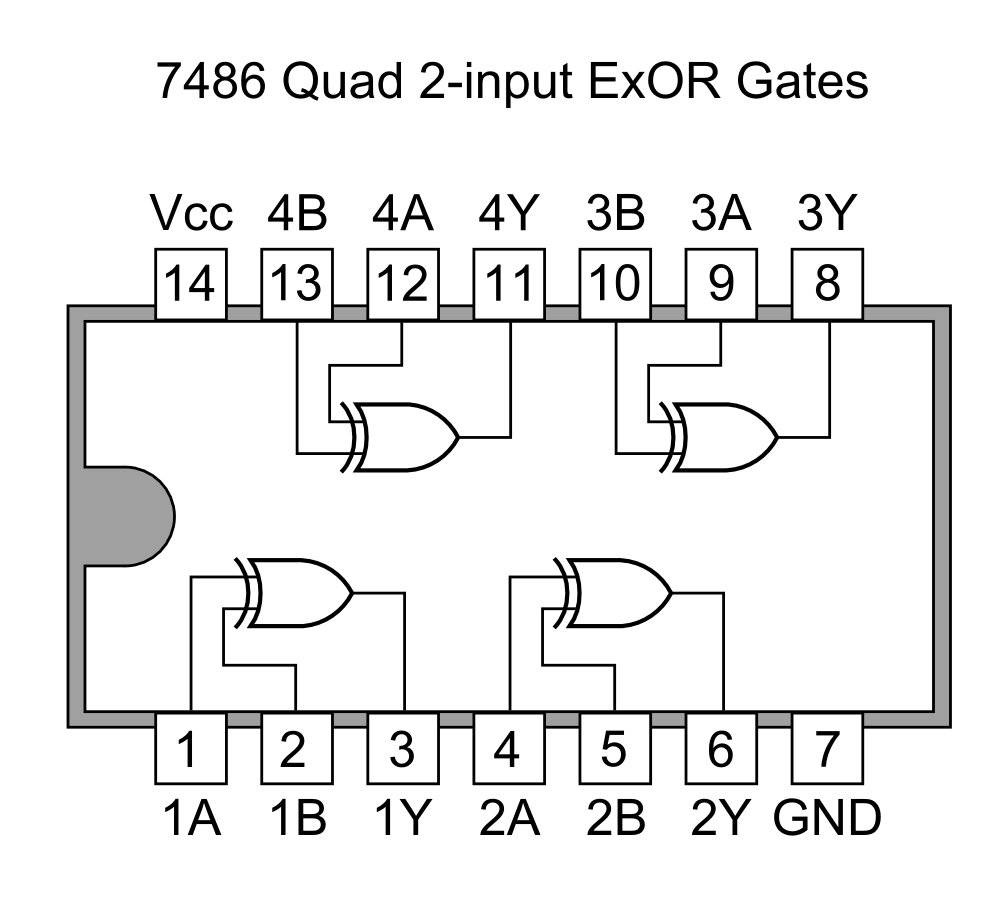
\includegraphics[scale=0.4]{7486.png}
\end{figure}

\subsection{Pin Diagram of IC74283}
\begin{figure}[H]
\centering
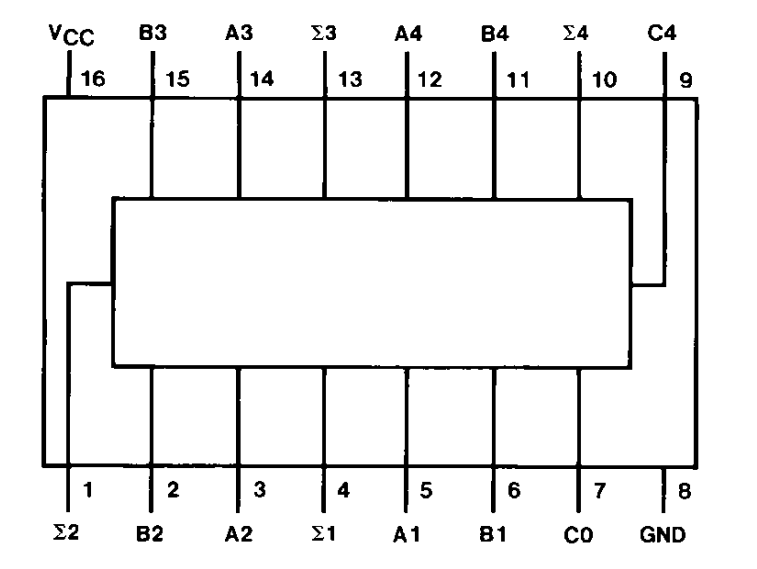
\includegraphics[scale=0.5]{IC74283.png}
\end{figure}

\section{Theory}neha.sathe@mitwpu.edu.in
\subsection{What is adder and Subtractor}
\subsection{Adder}
Adders are the combinatorial circuits which are used to add two binary numbers. The nature of the adders chosen depends on the characteristics of the binary numbers which need to be added. Say for example, if one needs to add two single bit binary digits, then one can use half adder while if there is an additional carry which needs to be added along with them, then one may resort to the use of full adder.
\subsection{Subtractor}
Subtraction of two binary numbers can be accomplished by adding 2's complement of the subtrahend to the minuend and disregarding the final carry if any. If the MSB bit in the result of addition is a '0'. then the result of addition is the correct answer. If the MSB bit is a '1'. , this implies that the answer has a negative sign. The true magnitude, in this case, is given by 2's complement of the result of the addition.
\subsection{Parallel Adder}
what if we want to add a binary number which has multiple bits in it. In such a case, the need arises to use a parallel adder. Parallel adder is nothing but a cascade of several full adders. The number of full adders used will depend on the number of bits in the binary digits which require to be added.
\begin{figure}[H]
\centering
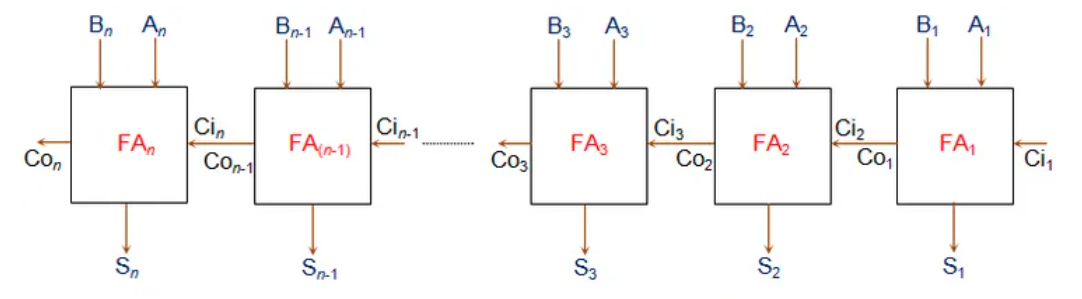
\includegraphics[scale=0.5]{parallel adder.png}
\caption{Parallel Adder}
\end{figure}
\subsection{Serial Adder}
A serial adder is abinary adder that is capable of forming sum and carry outputs for add end and augend words of greater than one bit in length. 
\begin{figure}[H]
\centering
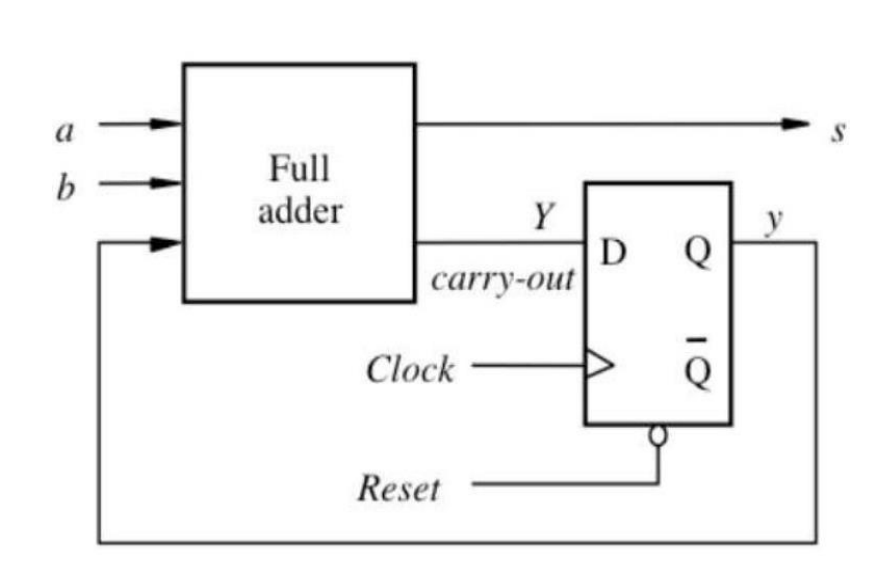
\includegraphics[scale=0.4]{serial adder.png}
\caption{Serial Adder}
\end{figure}
\subsection{Advantages of Parallel Adder to Serial Adder}
\begin{enumerate}
	\item A parallel Adder is faster.
	\item It uses registers with parallel load capacity
	\item The number of full adder circuits is equal to the number of bits in the binary adder. 
	\item It is a combinatioal Circuit. 
	\item Time required does not depend on the number of bits. 
	\item It is cheaper
\end{enumerate}
\subsection{Disadvantages of Parallel Adder to Serial Adder}
\begin{enumerate}
	\item Each adder has to wait for the carry which is to be generated from the previous
	adder in chain.
	\item The propagation delay( delay associated with the travelling of carry bit) is found to
	increase with the increase in the number of bits to be added.
\end{enumerate}
\section{Prodecure}
\begin{enumerate}
	\item Select the Right components and place them on the breadboard.
	\item Add power to the Circuit.
	\item Connect the Components using breadboard wires on tinkercad according to the drawn Circuit diagram.
	\item Input the numbers and Check its working.
\end{enumerate}

\section{Circuit Diagrams}
\subsection{Tinkercad Screenshots}
\begin{figure}[H]
\centering
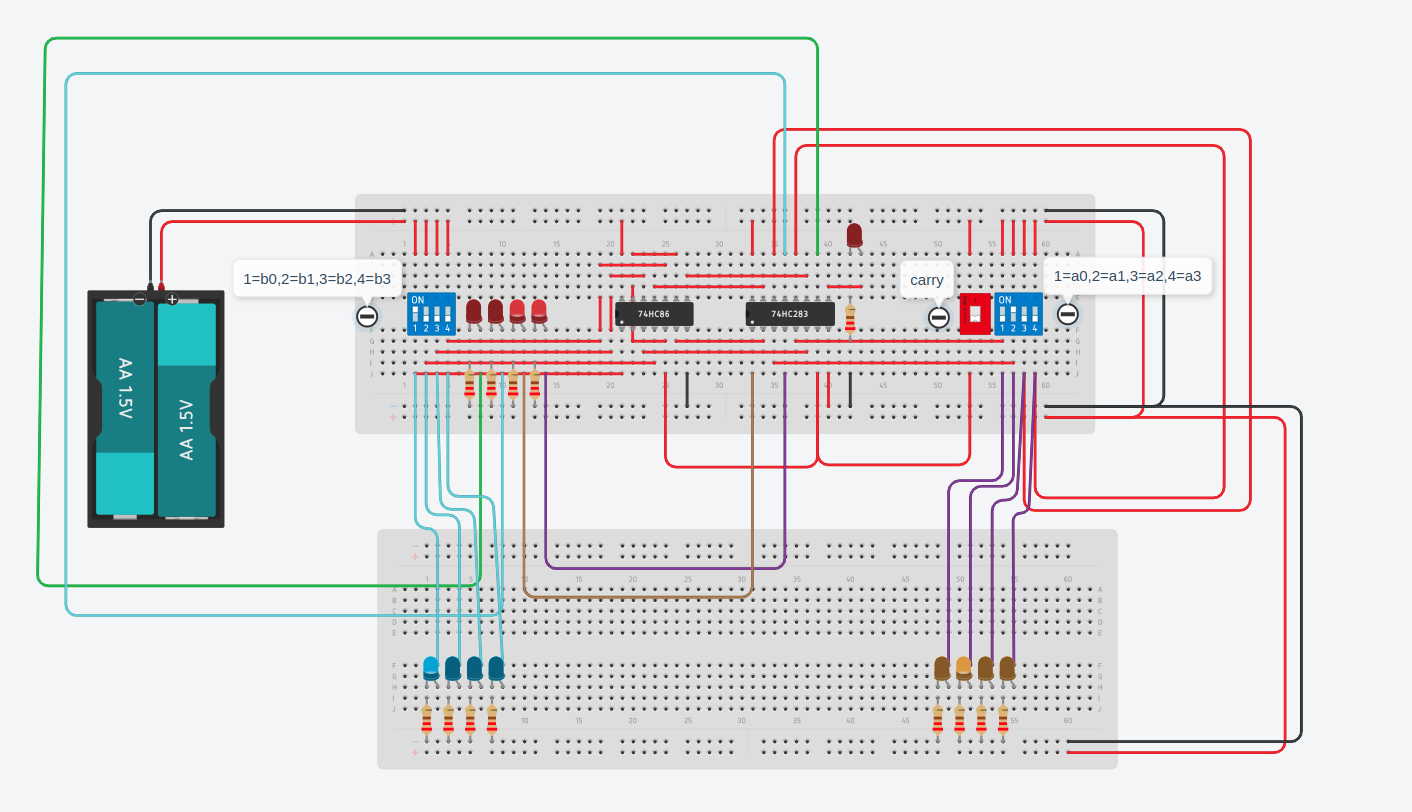
\includegraphics[scale=0.5]{tinkercad 1.png}
\caption{Adder Mode}
\end{figure}

\begin{figure}[H]
\centering
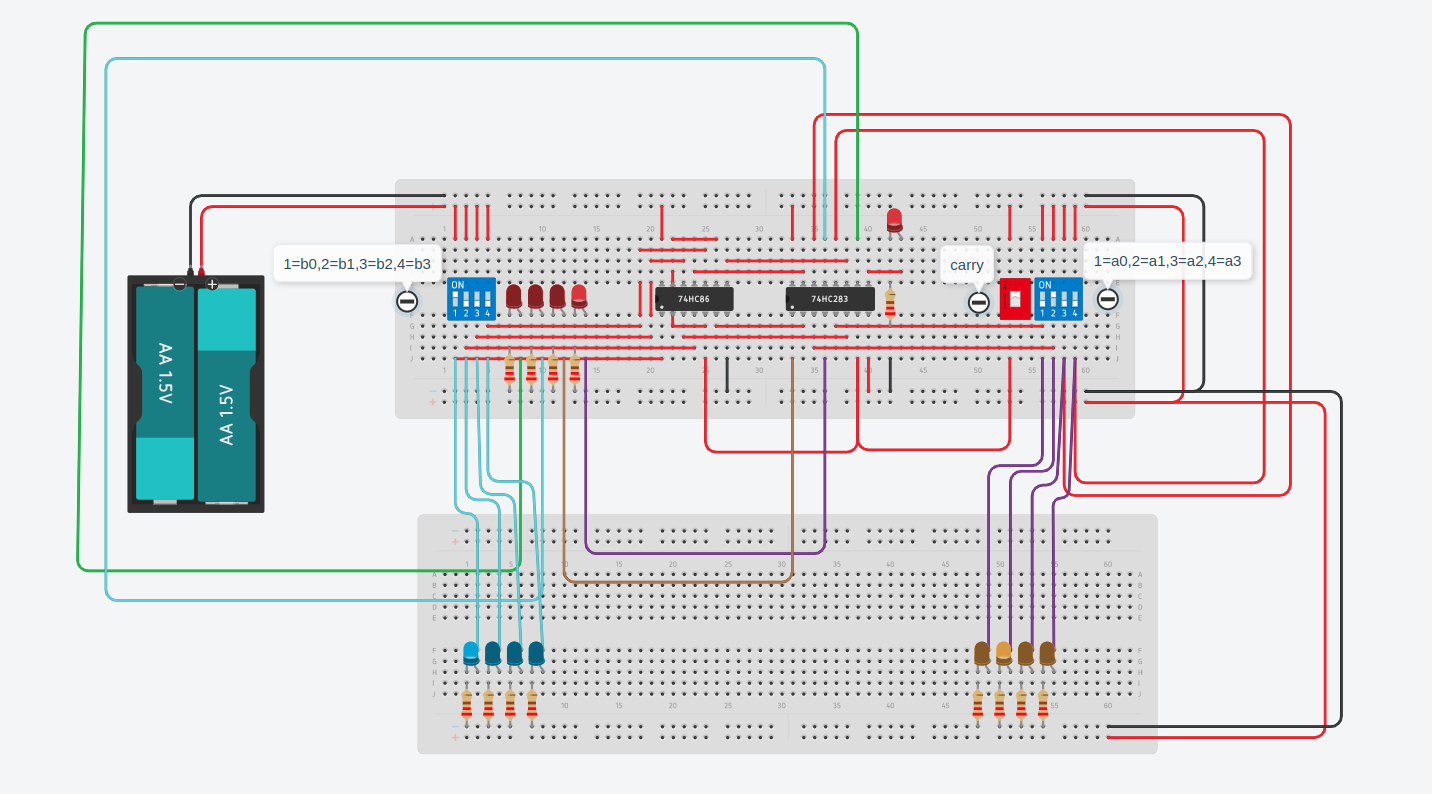
\includegraphics[scale=0.48]{tinkercad 2.png}
\caption{Subtractor Mode}
\end{figure}
\subsection{Logic Diagram}

\begin{figure}[H]
\centering
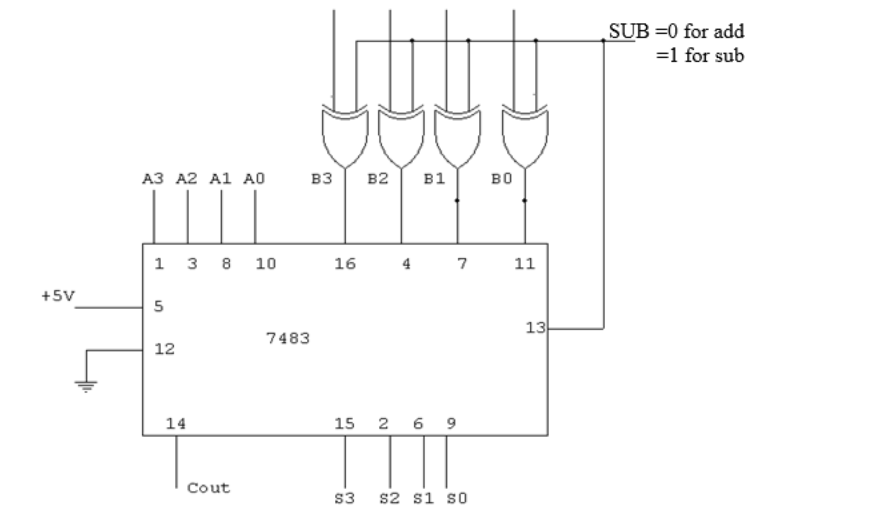
\includegraphics[scale=0.5]{logic.png}
\caption{}
\end{figure}

\subsection{Circuit Pin Diagram}
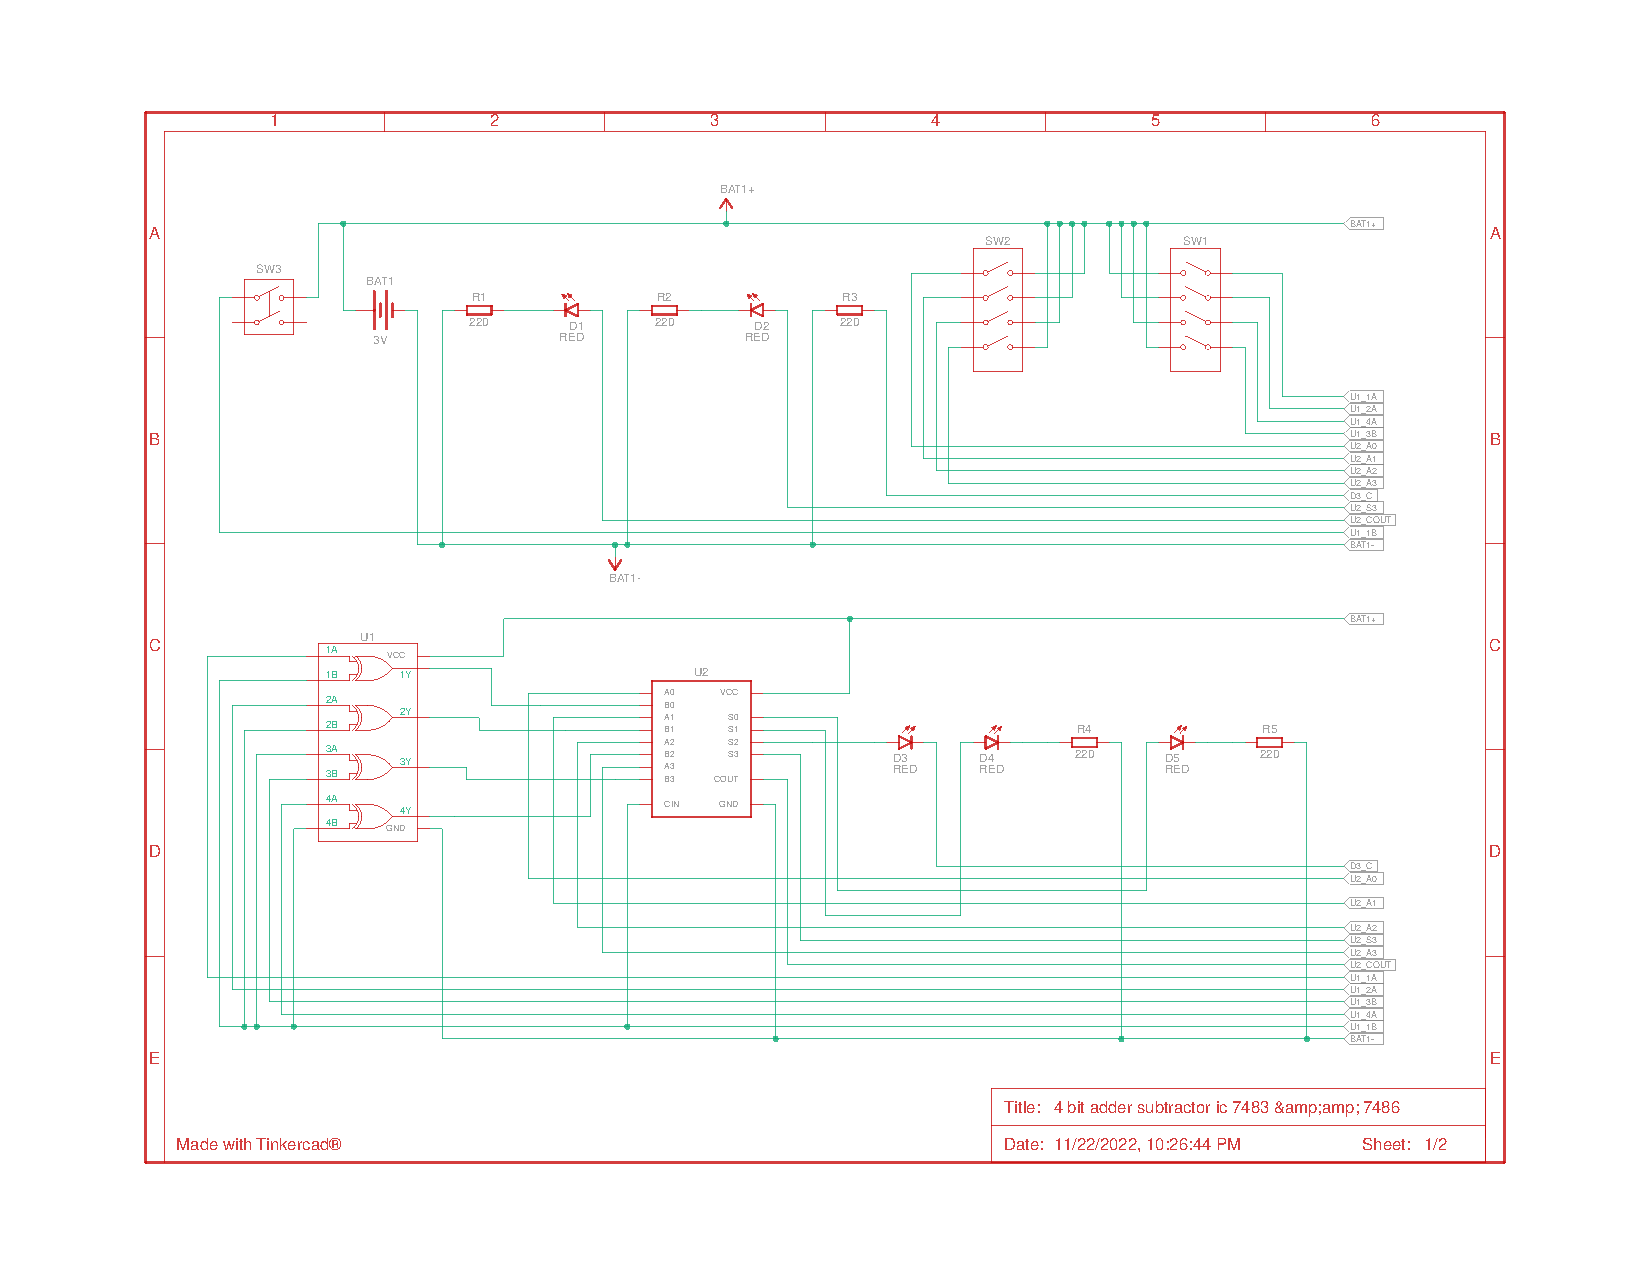
\includepdf{1.pdf}
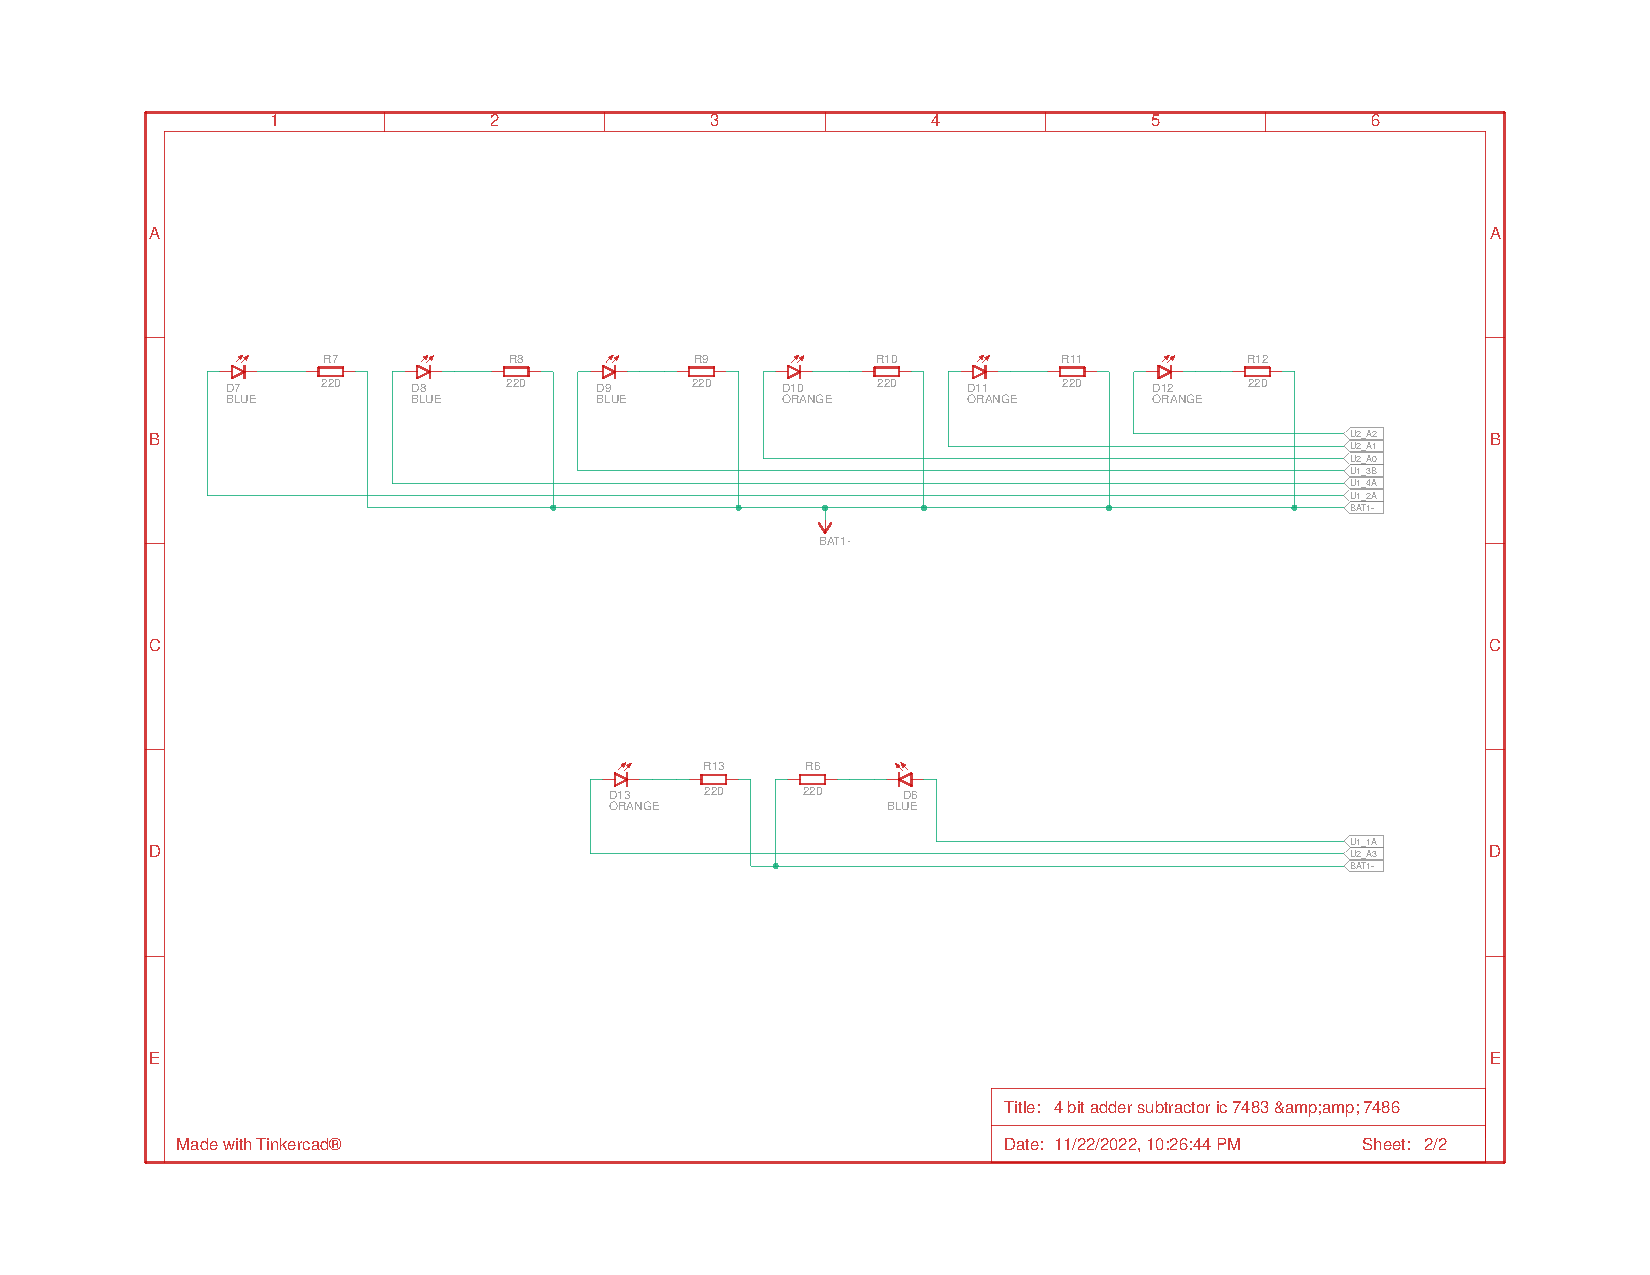
\includepdf{2.pdf}

\section{Applications}
\begin{enumerate}
	\item For performing arithmetic calculations in electronic calculators and other digital devices.
	\item In Timers and Program Counters.
	\item Useful in Digital Signal Processing.
	\item Suubtractors are widely used in in computer's ALU (Arithmetic logic unit) to compute addition as well as CPU (Central Processing unit) and GPU (Graphics Processing unit) for graphics applications to reduce the circuit complexity.
	\item Adder and subtractor are basically used for performing arithmetical functions like addition, subtraction, multiplication and division in electronic calculators and digital instruments.
	\item Adders are used in digital calculators for arithmetic addition and devises that uses some kind of increment or arithmetic process
	\item They are also used in microcontrollers for arithmetic additions, PC (program counter) and timers.
	\item It is also used in processors to calculate address, tables and similar operations
	\item It is also used in networking and DSP (Digital signal processor) oriented system
\end{enumerate}


\section{Conclusion}
Thus learnt how to implement a Full adder And a subtractor using IC7483. 
\end{document}
